\documentclass{../res/univ-projet}

%Import des packages utilisés pour le document
\usepackage[utf8x]{inputenc}
\usepackage[francais]{babel}
\usepackage[T1]{fontenc}

\usepackage{longtable}
\usepackage{../res/tikz-uml}

%Redéfinition des marges
\addtolength{\topmargin}{-1cm}
\addtolength{\textheight}{1cm}
\addtolength{\headsep}{0.8cm}
\addtolength{\footskip}{-0.2cm}

%Variables
\logo{../res/logo_univ.png}
\title{Document d'architecture du logiciel}
\author{Matthieu \bsc{Fin}, Guillaume \bsc{Leroy}}
\projet{Projet PGP}
\projdesc{Etude et implantation d'un outil graphique de gestion de clé PGP}
\filiere{Master 1 SSI }
\matiere{Conduite de projet}
\version{0.1}
\relecteur{Pierre \bsc{Balmelle}}
\signataire{Magali \bsc{Bardet}}
\date{\today}


\histentry{0.1}{23/11/2014}{Version initiale.}

% Definition de couleurs :
% Couleur de fond des nom de classes
\definecolor{classColor}{rgb}{.20,.42,.57}
% Couleur de fond des noms de méthode
\definecolor{methodeColor}{rgb}{.38,.62,.81}
% Couleur de fond des legends (Nom, Entrée, precondtion, sortie, postcondition, description)
\definecolor{legendColor}{rgb}{.45,.58,.67}

% Commande permettant de créer un tableau entrées / sortie / pré-post conditions pour les méthodes
% N'affiche pas les champs vides...
\newcommand{\methode}[6]{
  \def\vide{} \def\tempa{#1} \def\tempb{#2} \def\tempc{#3} \def\tempd{#4} \def\tempe{#5} \def\tempf{#6}
  \def\casa{\ifx\empty\tempa \else \hline \color{white}\cellcolor{legendColor}\bfseries{Nom}            & #1 \cr \fi }
  \def\casb{\ifx\empty\tempb \else \hline \color{white}\cellcolor{legendColor}\bfseries{Entrée}         & #2 \cr \fi }
  \def\casc{\ifx\empty\tempc \else \hline \color{white}\cellcolor{legendColor}\bfseries{Préconditions}  & #3 \cr \fi }
  \def\casd{\ifx\empty\tempd \else \hline \color{white}\cellcolor{legendColor}\bfseries{Sortie}         & #4 \cr \fi }
  \def\case{\ifx\empty\tempe \else \hline \color{white}\cellcolor{legendColor}\bfseries{Postconditions} & #5 \cr \fi }
  \def\casf{\ifx\empty\tempf \else \hline \color{white}\cellcolor{legendColor}\bfseries{Description}    & #6 \cr \fi }
  %\begin{tabular}{|>{\centering}p{2.5cm}|>{\centering}p{7cm}|}
  %\begin{tabular}{|>{\centering}p{2.5cm}|>{\centering}p{9cm}|}
  \begin{tabular}{|>{\centering}p{2.5cm}|>{\centering}p{10.5cm}|}
    \casa \casb \casc \casd \case \casf
    \hline
  \end{tabular}
}

% Commande pour definir une methode dans une \class
\newcommand{\methodeclass}[6]{
  & \color{white}\cellcolor{methodeColor}\bfseries{#1} & \cr
  & \methode{}{#2}{#3}{#4}{#5}{#6} & \cr
  & & \cr
}

% Commande permettant de regrouper des methode dans un tableau portant le nom de la classe.
\newcommand{\class}[2]{%
  \begin{longtable}{|c c c|}
    \hline
    \multicolumn{3}{|>{\centering\color{white}\columncolor{classColor}}p{\linewidth}|}{\bfseries{#1}} \endfirsthead%\cr
    \hline
    \multicolumn{3}{|>{\color{white}\columncolor{classColor}}c|}{\bfseries{#1} (suite ...)}\\
    & & \\
    \endhead
    \hline 
    \multicolumn{3}{|p{\linewidth}|}{Suite page suivante}
    \\ \hline \endfoot 
    %\hline
    \multicolumn{3}{|p{\linewidth}|}{Fin de la classe #1} \\
    \hline
    \endlastfoot \hline
    & & \cr
    #2
    \hline
  \end{longtable}
}


% -- Début du document -- %
\begin{document}

%Page de garde
\maketitle
\newpage
%La table des matières
\tableofcontents
\newpage

\section{Objet}
  Ce document permet d'établir une vue globale de l'architecture logicielle envisagée pour la conception d'une interface graphique reposant sur le logiciel GnuPG de façon à simpliciter son utilisation pour un utilisateur débutant, mais toutefois en laissant apparaitre les fonctionnalités avancées pour un utilisateur expérimenté. Il décrit comment concevoir cette interface pour répondre aux spécifications du client ainsi qu'une conception détaillée des différents modules nécessaires à son bon fonctionnement. 

\section{Documents applicables et de référence}
  \begin{itemize}
    \item La spécification technique des besoins
  \end{itemize}

\section{Terminologie et sigles utilisés}
  \subsection{Acronymes}
    \begin{itemize}
      \item GNOME GNU Network Object Model Environment
      \item GNU GNU's Not UNIX
      \item IETF Internet Engineering Task Force
      \item KDE K Desktop Environment
      \item MVC Model View Controller
      \item PGP Pretty Good Privacy
      \item RFC Request For Comments
    \end{itemize}

  \subsection{Glossaire}
    \begin{itemize}
      \item C++\\
        Langage de programmation compilé.
      \item Environement de bureau\\
        Ensemble de programmes qui permettent de manipuler le système à travers une interface graphique.
      \item MVC\\
        Patron de conception répondant aux besoins des applications interactives en séparant les problématiques en trois parties :
        \begin{itemize}
          \item Le modèle\\
            Il représente les données manipulées par l'application et est responsable de leur intégrité.
          \item La vue\\
            Ce avec quoi l'utilisateur interagit. Sa fonction principale est d'afficher les données envoyées par le modèle.
          \item Le controller\\
            Il traite les évènements et met à jour la vue ou le modèle selon l'action effectuée.
        \end{itemize}
      \item Qt\\
        Interface de programmation orientée objet développée en C++ permettant la conception simple d'interface graphique compatible GNU Linux / Windows / Mac OS X.
      \item Sémaphore : Un sémaphore est une variable (ou un type de donnée abstrait)
            et constitue la méthode utilisée couramment pour restreindre l'accès à des
            ressources partagées (par exemple un espace de stockage) dans un environnement
            de programmation concurrente.\\
            Sur un sémaphore trois action sont possibles :
            \begin{itemize}
               \item INIT(sem, val), qui initialise le sémaphore sem a la valeur val.
               \item P(sem) que l'on peut assimiler a la notion de prendre une ressource.
               \item V(sem) sue l'on peut assimiler a la notion de libérer une ressource.
             \end{itemize} 
      \item SHM : Shared Memory en français : Mémoire Partagée,
            est un moyen de partager des données entre différents processus :
            une même zone de la mémoire vive est accessible par plusieurs processus.
    \end{itemize}

\section{Configuration requise}
  \subsection{Système d'exploitation}
    GNU/Linux basé sur debian avec un noyau en version 3.14.29.
  \subsection{Logiciels}
    Environnement de bureau KDE (v4.0 ou ultérieure) ou GNOME (v3.0 ou ultérieure)\\
    GnuPG (v1.4 ou ultérieure)
  \subsection{Matériel}
    Aucune configuration minimale n'est demandée.

\section{Architecture statique}
  \subsection{Structure} % (fold)
    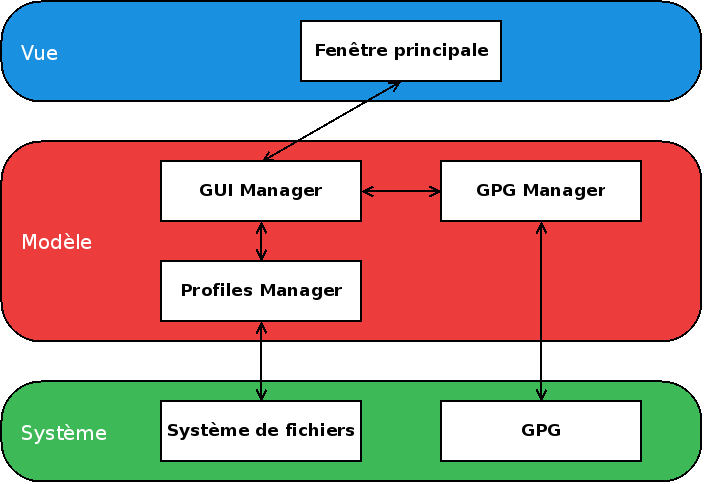
\includegraphics[scale=0.5]{graphics/diagramme_archi.png}
  \newpage

  \subsection{Composants principaux}
    
    \subsubsection{Fenêtre principale}

      La fenêtre principale est la partie du logiciel permettant d'afficher
      des informations a l'utilisateur et d'interagir avec ce dernier.

      La maquette retenu pour le style global de cette vue est la suivante :
      \begin{center}
        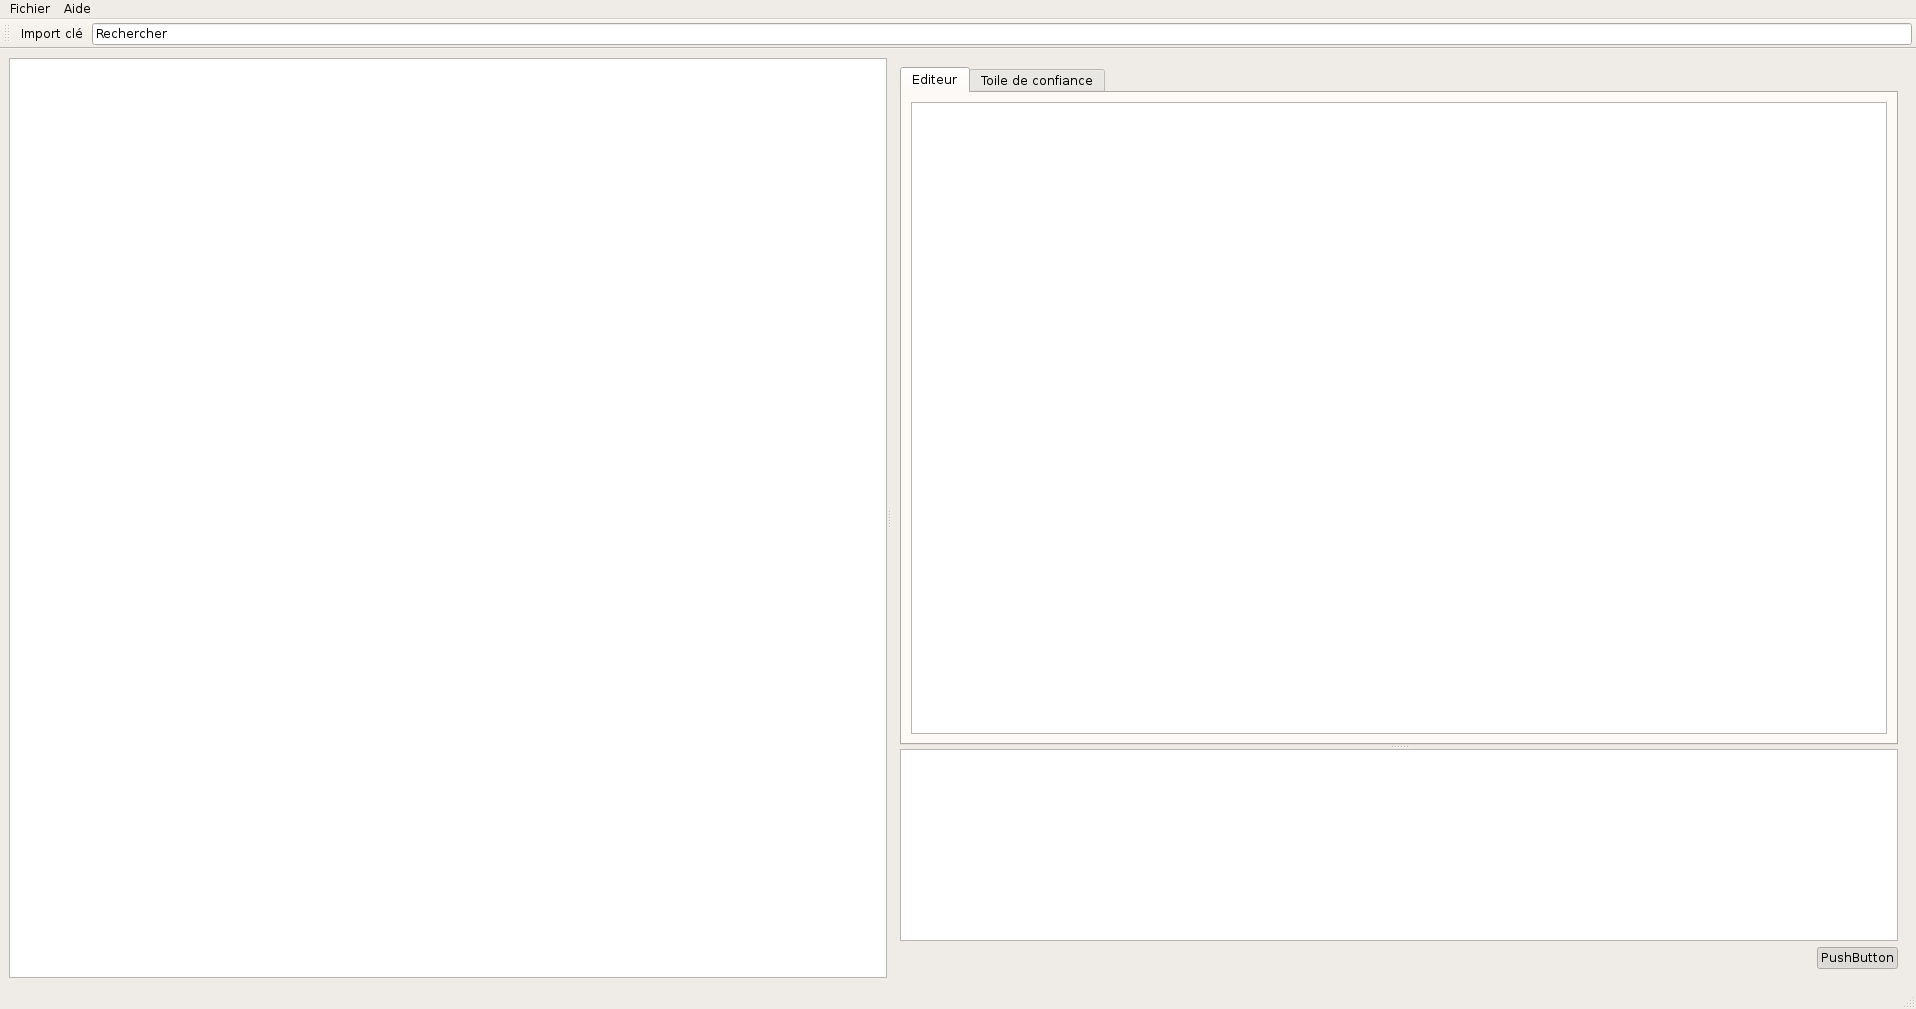
\includegraphics[scale=.25]{../res/maquette.png}
      \end{center}

      \begin{itemize}
        \item La partie supérieure présente une barre d'outils permettant de faire une recherche parmi les 
      clés présentes dans le trousseau de clés, ainsi qu'une barre de menu, permettant d'accéder à l'ensemble
      des fonctionnalités de l'application.
        \item La partie de gauche est un arbre qui permet de visualiser l'ensemble des clés présentes
        dans le trousseau ainsi qui de réaliser toutes les actions de modifications de clés (révocation, signature, ...)
        \item La partie de droite présente au choix un champ d'édition de texte permettant de chiffrer/déchiffrer
        du texte à la volée, ou bien le rendu graphique de la toile de confiance.
        \item La partie en bas a droite est une fenêtre qui affiche toutes les commandes GNUPG effectués
        par l'application ainsi que les retours de GNUPG.
      \end{itemize}

    \subsubsection{Un gestionnaire graphique}

      Le gestionnaire graphique représente en fait l'ensemble des modèles des vues,
      telles que le modèle d'une clé, les différents modèles nécessaire a la réalisation
      de la toile de confiance.

    \newpage
    \subsubsection{Un gestionnaire de profils}

      Pour répondre au besoin de pouvoir exécuter différentes instances de l'interface, ayant chacune
      un trousseau de clé gpg différent, nous utilisons un système de profils, c'est a ce composants
      de gérer un fichier de configuration de l'application qui permet de sauvegarder différents
      profils a savoir qu'un profil est constitué de :
      \begin{itemize}
        \item Un identifiant de profile.
        \item Un chemin vers l'exécutable de gpg (permettant d'avoir des profil utilisant des versions différentes de gpg).
        \item Un chemin vers un dossier de configuration de gpg (permettant d'avoir un trousseau de clés différents par profils).
      \end{itemize}
      De plus deux profils ne peuvent avoir le même identifiant de profil,
      ni le même chemin de configuration gpg.

      C'est ce composant qui permet de créer un profil, de changer de profil, ou de modifier un profil.
      C'est également lui qui s'occupe de s'assurer qu'un profil n'est actif qu'au plus une fois
      (c'est plus précisément la classe Launcher qui est charger de cette tâche dans notre implantation).

    \subsubsection{Un gestionnaire de gpg}

      C'est le composant qui permet la communications avec GNUPG,
      sachant qu'après étude il n'est pas toujours possible d'écrire ou de lire sur l'entrée/la sortie standard de GNUPG
      il faut préciser un mode d'affichage et un mode d'écriture a l'aide des options --status-fd=1 et --command-fd=0
      permettant ainsi pour les commandes gpg qui demandes un interaction de l'utilisateur d'afficher
      les données avec un format spécifique (permettant d'effectuer un parsing des réponses de GPG).
      Et en plus gpg affiche sa sortie sur sa sortie standard et non sur /dev/tty comme a sa fâcheuse habitude (de même pour son entrée).

      Ce composant doit donc ajouter ces options aux commandes demandées qui nécessite une interaction de l'utilisateur.

      Ainsi les modèles des vue qui nécessite une modification ou une requête à GNUGP demandera au gestionnaire de le faire
      en utilisant une notion d'action qui permet d'abstraire pour le reste de l'application le fait qu'une commande soit
      interactive ou non et toute la communication avec GNUPG.

      Cette communication s'effectue donc par la création d'un processus qui redirige son entrée standard et sa sortie standard
      sur des tube anonymes permettant ainsi au composant d'envoyer les données de la commande au processus et de récupérer la
      réponse du processus.


    \subsubsection{gpg ou GNUPG}

      C'est évidement une implantation open-source et complète du standard OpenPGP.
      L'application est pensée pour fonctionner avec la version 2.0.*.
      Mais il est possible de modifier le chemin d’accès a l’exécutable GNUPG.

      Sous GNU/Linux cette commande est généralement disponible dans les dépôts binaire de la distribution.
      Pour Windows il existe toutes sortes d'implantations équivalentes telles que "gpg4win" par exemple.


  \newpage
  \subsection{Patron d'architecture}

    L'application graphique reposant sur Qt, nous allons utiliser le patron d'architecture modèle-Vue
    reposant sur le fonctionnant des signaux de Qt :
    \begin{center}
    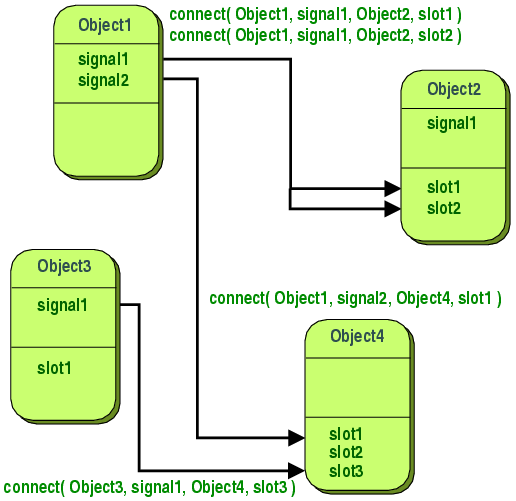
\includegraphics[scale=.5]{../res/MV.png}
    \end{center}

    Ainsi un signal est émit par un objet et réceptionné par un autre objet en exécutant une de ces méthodes
    qui est alors dénommé 'slot'.

  \subsection{Description des classes} % (fold)
      
    \begin{center}
    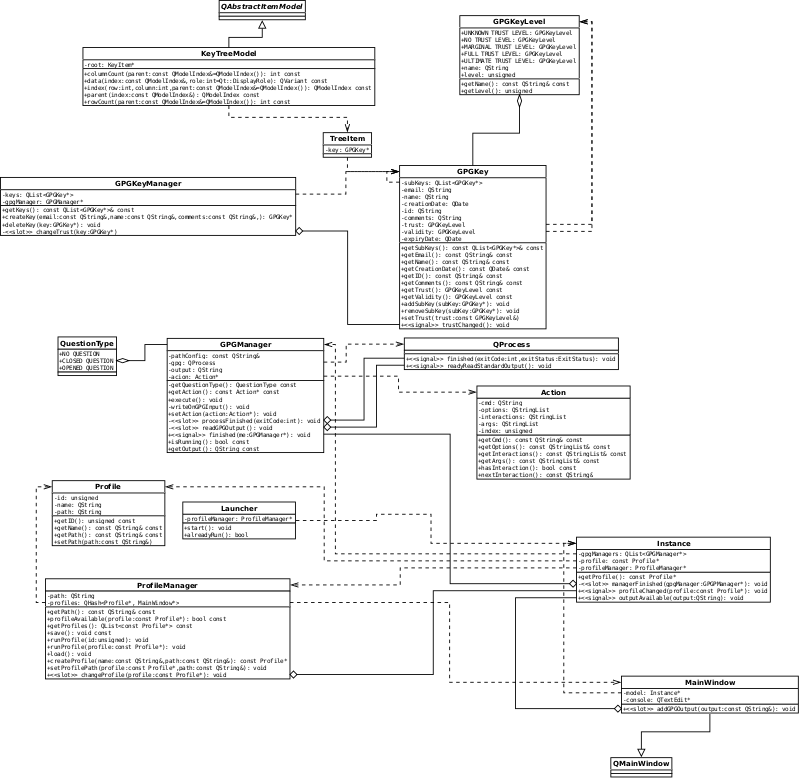
\includegraphics[scale=.5]{graphics/diagramme-classes.png}
    
    Ce diagramme de classe est disponible en \href{graphics/diagramme-classes.svg}{annexe} (en svg)
    et permet de visualiser les classes principales ainsi que les échanges principaux utilisant
    les signaux de Qt.
    \end{center}

      Dans la suite de cette section chacune de ces classes sont définies plus précisément.

      \subsubsection{Launcher}

        Cette classe est le point d'entrée de l'application, son unique rôle est de lancer des instances de l'application
        graphique en s'assurant qu'il n'y ait pas deux instances graphiques avec un profil utilisateur
        identique.
        
        Pour assurer l'unicité du processus gérant les instances graphiques, nous utilisons un SHM,
        sa présence permettant de signaler qu'un processus pour l'application est présent et attend
        d'y lire des données.
        
        Le SHM sera composé de deux sémaphores noté semW (pour les écrivains) et semR (pour le lecteur)
        voici le fonctionnement synthétisé du démarrage de l'application :

        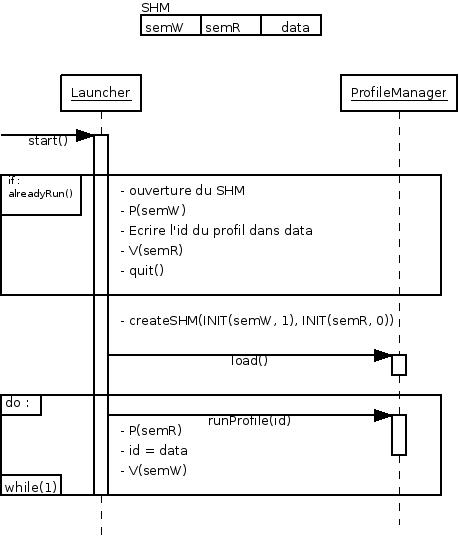
\includegraphics[scale=0.65]{graphics/launcherSequence.jpeg}

        \class{Launcher}{
          \methodeclass
            {start} % Nom
            {} % Entrée
            {} % Préconditions
            {} % Sortie
            {} % Postconditions
            {
            Permet de lancer l'application.\\
            Si elle est déja lancée, cette méthode permet de signifier au processus qu'une nouvelle instance
            de l'application est demandée.
            } % Description
            \methodeclass
              {alreadyRun} % Nom
              {} % Entrée
              {} % Préconditions
              {Booléen indiquant si un autre processus s'occupe déjà de lancer des instances graphiques ou non.} % Sortie
              {} % Postconditions
              {
                Permet de savoir si un processus gère les instances graphiques.\\
                Et si on doit écrire dans le SHM le profil à lancer ou le créer.
              } % Description
        }

      \subsubsection{Profile}
      
        \class{Profile}{
          \methodeclass
            {getID}
            {}
            {}
            {Entier représentant l'identifiant unique du profil}
            {}
            {Renvoie l'identifiant unique du profil}
          \methodeclass
            {getName}
            {}
            {}
            {QString représentant le nom du profil}
            {}
            {Renvoie le nom du profil}
          \methodeclass
            {getPath}
            {}
            {}
            {QString représentant le chemin absolu vers le dossier de configuration de GPG}
            {}
            {Renvoie le chemin absolu vers le dossier de configuration}
          \methodeclass
            {setPath}
            {path : QString}
            {path référence un dossier de configuration de GPG valide}
            {}
            {QString représentant le chemin vers le dossier de configuration de GPG du profil est changé}
            {Change le dossier de configuration de GPG du profil}
        }

      \subsubsection{ProfileManager}
        \class{ProfileManager}{
          \methodeclass
          {getPath}
          {}
          {}
          {QString représentant le chemin absolu vers le fichier de configuration de l'application}
          {}
          {Renvoie le chemin absolu vers le fichier de configuration de l'application}
        
          \methodeclass
          {profileAvailable}
          {p : Profile}
          {}
          {Booléen ayant pour valeur vrai si p est libre d'utilisation, faux sinon}
          {Vrai si p n'est utilisé par aucune autre fenêtre de l'application}
          {Renvoie vrai si p est libre, faux sinon}
          
          \methodeclass
          {getProfiles}
          {}
          {}
          {La liste de tous les profils}
          {QList<Profile> contenant tous les profils présents dans le fichier de configuration de l'application}
          {La liste de tous les profils présents dans le fichier de configuration de l'application}
          
          \methodeclass
          {save}
          {}
          {}
          {}
          {La liste des profils est sauvegardée dans le fichier de configuration de l'application}
          {Sauvegarde la liste des profils dans le fichier de configuration de l'application}
          
          \methodeclass
          {runProfile}
          {id : Entier}
          {id est positif ou nul, il correspond à un identifiant de profil et ce profil doit être libre d'utilisation}
          {}
          {Une nouvelle fenêtre est ouverte avec le profil ayant pour identifiant id}
          {Ouvre une nouvelle fenêtre avec le profil donné}

          \methodeclass
          {load}
          {}
          {}
          {}
          {Les profils présents dans le fichier de configuration de l'application sont chargés}
          {Charge les profils présents dans le fichier de configuration de l'application}
          
          \methodeclass
          {createProfile}
          {name : QString\\path : QString}
          {name n'est pas vide\\path référence un dossier de configuration de GPG valide}
          {Profile représentant le profil créé}
          {Un objet Profile est créé et il est ajouté à la liste des profils}
          {Crée un profil, l'ajoute à la liste des profils et retourne l'objet Profil créé}
          
          \methodeclass
          {setProfilePath}
          {p : Profile\\path : QString}
          {path est un chemin absolu référençant un dossier de configuration de GPG valide}
          {}
          {Le chemin de p est changé}
          {Change le dossier de configuration lié à p}
          
          \methodeclass
          {changeProfile}
          {p : Profile}
          {p est un profil libre d'utilisation}
          {}
          {Le profil de la fenêtre courante est changé}
          {Change le profil associé à la fenêtre courante}
        }
      \subsubsection{Action}
        \class{Action}{
          \methodeclass
          {getCmd}
          {}
          {}
          {QString représentant le nom de la commande GPG}
          {}
          {Retourne le nom de la commande GPG}
          
          \methodeclass
          {getOptions}
          {}
          {}
          {QStringList contenant les options de la commande GPG}
          {}
          {Retourne la liste des options de la commande GPG}
          
          \methodeclass
          {getInteractions}
          {}
          {}
          {QStringList contenant les intéractions utilisateur durant l'exécution de la commande}
          {}
          {Retourne la liste des intéractions utilisateur durant l'exécution de la commande}
          
          \methodeclass
          {getArgs}
          {}
          {}
          {QStringList content les arguments de la commande GPG}
          {}
          {Retourne la liste des arguments de la commande GPG}
          
          \methodeclass
          {hasInteraction}
          {}
          {}
          {Booleen ayant pour valeur vrai s'il reste des interactions utilisateur}
          {}
          {Retourne vrai s'il reste des interactions utilisateur}
          
          \methodeclass
          {nextInteraction}
          {}
          {hasInteraction()}
          {QString représentant l'interaction utilisateur courante}
          {L'interaction utilisateur courante devient l'interaction utilisateur suivante}
          {Retourne l'interaction utilisateur suivante}
        }
        
        \subsubsection{QuestionType}
        Énumération des différents types de questions :
        \begin{itemize}
          \item NO\_QUESTION
          \item CLOSED\_QUESTION
          \item OPENED\_QUESTION
        \end{itemize}
        
        \subsubsection{GPGManager}
          \class{GPGManager}{
          \methodeclass
          {isRunning}
          {}
          {}
          {Boolean ayant pour valeur vrai si l'exécution de l'action par GPG est en cours}
          {}
          {Retourne vrai si l'exécution de l'action par GPG est en cours}
          
          \methodeclass
          {getQuestionType}
          {}
          {isRunning()}
          {QuestionType représentant le type de la dernière question posée par GPG}
          {}
          {Retourne le type de la dernière question posée par GPG}
          
          \methodeclass
          {getAction}
          {}
          {}
          {Action représentant l'action à exécuter par GPG}
          {}
          {Retourne l'action à exécuter par GPG}
          
          \methodeclass
          {execute}
          {}
          {!isRunning()}
          {}
          {GPG a exécuté l'action associée au manager}
          {Exécute l'action associé au manager}
          
          \methodeclass
          {setAction}
          {a : Action}
          {!isRunning()}
          {}
          {L'action associée au manager a été changé}
          {Change l'action à exécuter par GPG associée au manager}
        
          \methodeclass
          {getOutput}
          {}
          {!isRunning()}
          {QString représentant la sortie de GPG}
          {Contient la sortie de GPG}
          {Retourne la sortie de GPG}
        }
        
        \subsubsection{Instance}
          \class{Instance}{
            \methodeclass
            {getProfile}
            {}
            {}
            {Profile}
            {}
            {Retourne le profil associé à l'instance}
          }
          
        \subsubsection{GPGKeyLevel}
          \class{GPGKeyLevel}{
            \methodeclass
            {getName}
            {}
            {}
            {QString représentant le nom du niveau}
            {}
            {Retourne le nom du niveau}
            
            \methodeclass
            {getLevel}
            {}
            {}
            {Entier représentant le niveau}
            {}
            {Retourne le niveau}
          }
          
        \subsubsection{GPGKey}
          \class{GPGKey}{
          \methodeclass
          {getSubKeys}
          {}
          {}
          {QList<GPGKey> contenant les sous clés de cette clé}
          {}
          {Retourne la liste des sous clés de cette clé}
          
          \methodeclass
          {getEmail}
          {}
          {}
          {QString représentant l'email associé à la clé}
          {}
          {Retourne l'email associé à la clé}
          
          \methodeclass
          {getName}
          {}
          {}
          {QString représentant le nom du propriétaire de la clé}
          {}
          {Retourne le nom du propriétaire de la clé}
          
          \methodeclass
          {getCreationDate}
          {}
          {}
          {QDate représentant la date de création de la clé}
          {}
          {Retourne la date de création de la date}
          
          \methodeclass
          {getID}
          {}
          {}
          {QString représentant l'ID de la clé}
          {}
          {Retourne l'ID de la clé}
          
          \methodeclass
          {getComments}
          {}
          {}
          {QString représentant les commentaires de la clé}
          {}
          {Retourne les commentaires de la clé}
          &&\\
          \methodeclass
          {getTrust}
          {}
          {}
          {GPGKeyLevel représentant le niveau de confiance de la clé}
          {}
          {Retourne le niveau de confiance de la clé}
          
          \methodeclass
          {getValidity}
          {}
          {}
          {GPGKeyLevel représentant le niveau de validité de la clé}
          {}
          {Retourne le niveau de validité de la clé}
          
          \methodeclass
          {addSubKey}
          {k : GPGKey}
          {}
          {}
          {}
          {Ajoute une sous clé à cette clé}
          
          \methodeclass
          {removeSubKey}
          {k : GPGKey}
          {k est une sous clé de cette clé}
          {}
          {}
          {Supprime k des sous clés de cette clé}
          
          \methodeclass
          {setTrust}
          {t : GPGKeyLevel}
          {}
          {}
          {Le niveau de confiance de cette clé vaut t}
          {Change le niveau de confiance de cette clé}
        }
          
        \subsubsection{GPGKeyManager}
          \class{GPGKeyManager}{
            \methodeclass
            {getKeys}
            {}
            {}
            {QList<GPGKey> contenant toutes les clés appartenant au trousseau}
            {}
            {Retourne la liste de toutes les clés appartenant au trousseau}
            
            \methodeclass
            {createKey}
            {email : QString\\name : QString\\comments : QString}
            {}
            {GPGKey}
            {Une clé est crée et elle est ajoutée au trousseau}
            {Génére une clé, l'ajoute au trousseau et la retourne}
            
            \methodeclass
            {deleteKey}
            {k : GPGKey}
            {k fait partie du trousseau}
            {}
            {}
            {Supprime une clé du trousseau}
        }
           
  % subsection justification_techniques (end)
\section{Fonctionnement dynamique} % (fold)
\label{sec:fonctionnement_dynamique}

  \textcolor{blue}{
    TODO : \\
    Pour les principaux scénarii identifiés dans la spécification technique de besoin.
    \begin{itemize}
      \item Liste des composants mis en jeu.
      \item Description du processus de mise en oeuvre sous la forme d'une
      séquence d'appels aux services offerts par les différents composants et en faisant
      clairement apparaître :
      \begin{itemize}
        \item la logique et le flux des événements traités
        \item les interactions du logiciels avec les acteurs
        \item les interactions entre les composants au travers de leurs interfaces
      \end{itemize}
    \end{itemize}
  }
  \subsection{Exécution d'actions GPG}
  \begin{center}
    \begin{tikzpicture}
      \begin{umlseqdiag}
        \umlactor[class=Acteur]{acteur}
        \umlobject[class=MainWindow]{mainwindow}
        \umlobject[class=Instance]{instance}
        \begin{umlcall}[op=validate(), type=synchron]{acteur}{mainwindow}
          \umlcreatecall[class=Action, x=10]{mainwindow}{action}
          \begin{umlcall}[op=doAction(action), type=synchron, return=outputAvailable(output)]{mainwindow}{instance}
            \umlcreatecall[class=GPGManager, x=14]{instance}{manager}
            \begin{umlcall}[op=execute(), type=synchron, return=finished(this)]{instance}{manager}
            \end{umlcall}
            \begin{umlcall}[op=getOutput(), type=synchron, return=output]{instance}{manager}
            \end{umlcall}
          \end{umlcall}
          \begin{umlcallself}[op=addOutput(output), type=synchron]{mainwindow}
          \end{umlcallself}
        \end{umlcall}
      \end{umlseqdiag}
    \end{tikzpicture}
  \end{center}



  \subsubsection{Methode execute de GPGManager}
  \begin{center}
    \begin{tikzpicture}
      \begin{umlseqdiag}
        \umlobject[class=Instance]{instance}
        \umlobject[class=GPGManager]{manager}
        \umlobject[class=Action]{action}
        \umlobject[class=QProcess]{gpg}
        \begin{umlcall}[op=execute(), type=synchron]{instance}{manager}
          \begin{umlcall}[op=getArgs(), return=args]{manager}{action}
          \end{umlcall}
          \begin{umlcall}[op=start(pathExec{,} args), return=finished()]{manager}{gpg}
            \begin{umlcall}[op=readyReadStandardOutput()]{gpg}{manager}
            \end{umlcall}
            \begin{umlcall}[op=readAllStandardOutput()]{manager}{gpg}
              
            \end{umlcall}
          \end{umlcall}
        \end{umlcall}
      \end{umlseqdiag}
    \end{tikzpicture}
  \end{center}




% section fonctionnement_dynamique (end)
\section{Traçabilité} % (fold)
\label{sec:tra_abilit_}

  \textcolor{blue}{
    TODO : \\
    Récapitulatif des liens de dépendance entre les constituants du logiciel et les exigences de
    la STB (par exemple sous forme de tableau).
  }
  
\section{Attaque sur les Keys ID}
\subsection{Présentation}
Lorsque l'on envoie une clé sur un serveur, un "ID" est calculé pour permettre à ce dernier 
de rechercher beaucoup plus vite les clés demandés. Pour cela, il exécute une fonction de hashage, nommé SHA-1,
sur cette clé et gardent seulement les 4 ou 8 octets. Or, nous disposons maintenant d'une assez grande 
puissance de calcul pour pouvoir trouver des collisions sur les ID de 4 octets.
\subsection{Méthode de réalisation}
Notre attaque est de type bruteforce : on calcule une clé RSA et on modifie un ou plusieurs de ses champs (date de création, email...)
jusqu'à obtenir l'ID de la clé donnée.

% section tra_abilit_ (end)
\end{document}

